\documentclass{article}
\usepackage{fancyhdr}
\usepackage{amsthm}
\usepackage{etoolbox}
\usepackage{verbatim}
\usepackage{enumerate}
\usepackage{amsmath}
\usepackage{algorithmicx}
\usepackage{algorithm}
\usepackage{algpseudocode}
\usepackage{amssymb}
\usepackage{tikz}
	
\pagestyle{fancy}
\title{Chapter 19}
\author{Michelle Bodnar, Andrew Lohr}

\newcounter{curnum}
\setcounter{curnum}{0}

\newtheorem{th1}{Exercise} 
\newcommand{\calH}{\mathcal{H}}
\newcommand{\calX}{\mathcal{X}}
\newcommand{\calA}{\mathcal{A}}
\newcommand{\calY}{\mathcal{Y}}

\begin{document}
\maketitle


\noindent\textbf{Exercise 19.2-1}\\

Frst, we take the subtrees rooted at 24, 17, and 23 and add them to the root list. Then, we set H.min to 18. Then, we run consolidate. First this has its degree 2 set to the subtree rooted at 18. Then the degee 1 is the subtree rooted at 38. Then, we get a repeadted subtree of degree 2 when we consider the one rooted at 24. So, we make it a subheap by placing the 24 node under 18. Then, we consider the heap rooted at 17. This is a repeat for heaps of degree 1, so we place the heap rooted at 38 below 17. Lastly we consider the heap rooted at 23, and then we have that all the different heaps have distinct degrees and are done, setting H.min to the smallest, that is, the one rooted at 17.

The three heaps that we end up with in our root list are:

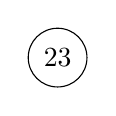
\begin{tikzpicture}[level/.style={sibling distance=30mm/#1}]
\node [circle,draw] (a){23}
;
\end{tikzpicture}

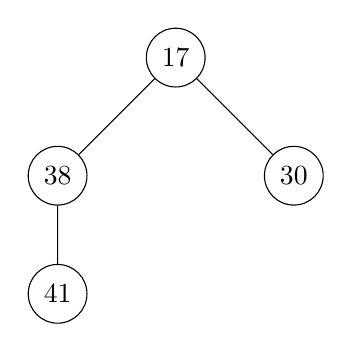
\begin{tikzpicture}[level/.style={sibling distance=30mm/#1}]
\node [circle,draw] (a){17}
  child {
  node [circle,draw] (b) {38}
  child{
  node [circle,draw] (c) {41}
  }
  }
  child {
  node [circle,draw] (d) {30}
  }
;
\end{tikzpicture}

and

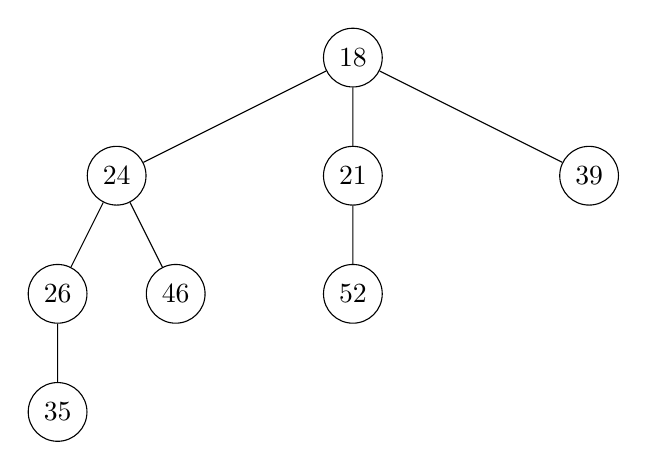
\begin{tikzpicture}[level/.style={sibling distance=30mm/#1}]
\node [circle,draw] (a){18}
  child{
node [circle,draw] (e){24}
  child {
  node [circle,draw] (f) {26}
  child{
  node [circle,draw] (g) {35}
  }
  }
  child {
  node [circle,draw] (h) {46}
  }
    }
  child {
  node [circle,draw] (b) {21}
  child{
  node [circle,draw] (c) {52}
  }
  }
  child {
  node [circle,draw] (d) {39}
  }
;
\end{tikzpicture}

\noindent\textbf{Exercise 19.3-1}\\

A root in the heap became marked because it at some point had a child whoose key was decreased. It doesn't add the potential for having to do any more actual work for it to be marked. This is because the only time that markedness is checked is in line 3 of cascading cut. This however is only ever run on nodes whoose parent is non NIL. Since every root has NIL as it parent, line 3 of cascadinc cut will never be run on this mared root. It will still cause the potential function to be larger than needed, but that extra computation that was paid in to get the potential function higher will never be used up later.\\

\noindent\textbf{Exercise 19.3-2}\\

Recall that the actual cost of FIB-HEAP-DECREASE-KEY is $O(c)$, where $c$ is the number of calls made to CASCADING-CUT.  If $c_i$ is the number of calls made on the $i^{th}$ key decrease, then the total time of $n$ calls to FIB-HEAP-DECREASE-KEY is $\sum_{i=1}^n O(c_i)$.  Next observe that every call to CASCADING-CUT moves a node to the root, and every call to a root node takes $O(1)$.  Since no roots ever become children during the course of these calls, we must have that $\sum_{i=1}^n c_i = O(n)$.  Therefore the aggregate cost is $O(n)$, so the average, or amortized, cost is $O(1)$. \\

\noindent\textbf{Exercise 19.4-1}\\

Add three nodes then delete one. This gets us a chain of length 1. Then, add three nodes, all with smaller values than the first three, and delete one of them. Then, delete the leaf that is only at depth 1. This gets us a chain of length 2. Then, make a chain of length two using this process except with all smaller keys. Then, upon a consolidate being forced, we will have that the remaining heap will have one path of length 3 and one of length 2, with a root that is unmarked. So, just run decrease key on all of the childeren along the shorter path, starting with those of shorter depth. Then, extract min the appropriate number of times. Then what is left over will be just a path of length 3. We can continue this process ad infinitum. It will result in a chain of arbitrarily long length where all but the leaf is marked. It will take time exponential in $n$, but that's none of our concern. 

More formally, we will make the following procedure $linear(n,c)$ that makes heap that is a linear chain of $n$ nodes and has all of its keys between $c$ and $c+2^n$. Also, as a precondition of running $linear(n,c)$, we have all the keys currently in the heap are less than $c$. As a base case, define $linear(1,c)$ to be the command insert(c). Define $linear(n+1,c)$ as follows, where the return value list of nodes that lie on the chain but aren't the root

$
\begin{array}{l}
S_1 = linear(n,c)\\
S_2 = linear(n,c+2^n)\\
x.key = -\infty\\
insert(x)\\
extractmin()\\
\text{ for each entry in $S_1$, delete that key}\\
\text{ The heap now has the desired structure, return $S_2$}\\
\end{array}
$\\

\noindent\textbf{Exercise 19.4-2}\\

Following the proof of lemma 19.1, if $x$ is any node if a Fibonacci heap, $x.degree = m$, and $x$ has children $y_1, y_2, \ldots, y_m$, then $y_1.degree \geq 0$ and $y_i.degree \geq i-k$.  Thus, if $s_m$ denotes the fewest nodes possible in a node of degree $m$, then we have $s_0 = 1, s_1 = 2, \ldots, s_{k-1} = k$ and in general, $s_m = k + \sum_{i=0}^{m-k}s_i$.  Thus, the difference between $s_{m}$ and $s_{m-1}$ is $s_{m-k}$.  Let $\{f_m\}$ be the sequence such that $f_m = m+1$ for $0 \leq m < k$ and $f_m = f_{m-1} + f_{m-k}$ for $m \geq k$. If $F(x)$ is the generating function for $f_m$ then we have $F(x) = \frac{1-x^k}{(1-x)(1-x-x^k)}$.  Let $\alpha$ be a root of $x^k = x^{k-1} + 1$.  We'll show by induction that $f_{m+k} \geq \alpha^m$.  For the base cases:

\begin{align*} 
f_k &= k+1 \geq 1 = \alpha^0 \\
 f_{k+1} &= k+3 \geq \alpha^1 \\
&\vdots \\
f_{k+k} &= k + \frac{(k+1)(k+2)}{2}  = k + k + 1 + \frac{k(k+1)}{2} \geq 2k + 1 + \alpha^{k-1} \geq \alpha^k.
\end{align*}

In general, we have
\[ f_{m+k} = f_{m+k-1} + f_m \geq \alpha^{m-1} + \alpha^{m-k} = \alpha^{m-k}(\alpha^{k-1} + 1) = \alpha^m.\]

Next we show that $f_{m+k} = k + \sum_{i=0}^m f_i$.  The base case is clear, since $f_k = f_0 + k = k+1$.  For the induction step, we have
\[ f_{m+k} = f_{m-1-k} + f_{m} = k + \sum_{i=0}^{m-1}f_i + f_m =  k + \sum_{i=0}^{m}f_i .\]

Observe that $s_i \geq f_{i+k}$ for $0 \leq i < k$.  Again, by induction, for $m \geq k$ we have
\[ s_m = k + \sum_{i=0}^{m-k} s_i \geq k + \sum_{i=0}^{m-k} f_{i+k} \geq k + \sum_{i=0}^{m} f_i = f_{m+k} \]
so in general, $s_m \geq f_{m+k}$.  Putting it all together, we have:
\begin{align*}
size(x) &\geq s_m \\
& \geq k + \sum_{i=k}^m s_{i-k} \\
&\geq k + \sum_{i=k}^m f_i \\
&\geq f_{m+k} \\
&\geq \alpha^m.
\end{align*}

Taking logs on both sides, we have 
\[ \log_{\alpha} n \geq m.\]
In other words, provided that $\alpha$ is a constant, we have a logarithmic bound on the maximum degree. \\


\noindent\textbf{Problem 19-1}\\

\begin{enumerate}[a.]
\item It can take actual time proportional to the number of children that x had because for each child, when placing it in the root list, their parent pointer needs to be updated to be NIL instead of x.

\item Line 7 takes actual time bounded by x.degree since updating each of the children of x only takes constant time. So, if $c$ is the number of cascading cuts that are done, the actual cost is $O(c+x.degree)$.

\item From the cascading cut, we marked at most one more node, so, $m(H') \le 1 + m(H)$ regardless of the number of calls to cascading cut, because only the highest thing in the chain of calls actually goes from unmarked to marked. Also, the number of children increases by the number of children that $x$ had, that is $t(H') = x.degree + t(H)$. Putting these together, we get that
\[
\Phi(H') \le t(H)+ x.degree + 2(1+m(H))
\]

\item The asymptotic time is $\Theta(x.degree) = \Theta(\lg(n))$ which is the same ayptotic time that was required for the originial deletion method.

\end{enumerate}

\noindent\textbf{Problem 19-2}\\

a. We proceed by induction to prove all four claims simultaneously.  When $k=0$, $B_0$ has $2^0 = 1$ node. The height of $B_0$ is 0. The only possible depth is 0, at which there are ${0 \choose 0} = 1$ node.  Finally, the root has degree 0 and it has no children.  Now suppose the claims hold for $k$.  $B_{k+1}$ is formed by connecting two copies of $B_k$, so it has $2^k + 2^k = 2^{k+1}$ nodes. The height of the tree is the height of $B_k$ plus 1, since we have added an extra edge connecting the root of $B_k$ to the new root of the tree, so the height is $k+1$.  At depth $i$ we get a contribution of ${k \choose i-1}$ from the first tree, and a contribution of ${k \choose i}$ from the second.  Summing these and applying a common binomial identity gives ${k+1 \choose i}$. Finally, the degree of the root is the sum of 1, and the degree of the root of $B_k$, which is $1+ k$. If we number the children left to right by $k, k-1, \ldots, 0$, then the first child corresponds to the root of $B_k$ by definition. The remaining children correspond to the proper roots of subtrees by the induction hypothesis. \\

b. Let $n.b$ denote the binary expansion of $n$.  The fact that we can have at most one of each binomial tree corresponds to the fact that we can have at most 1 as any digit of $n.b$.  Since each binomial tree has a size which is a power of 2, the binomial trees required to represent $n$ nodes are uniquely determined.  We include $B_k$ if and only if the $k^{th}$ position of $n.b$ is 1.  Since the binary representation of $n$ has at most $\lfloor \lg n \rfloor + 1$ digits, this also bounds the number of trees which can be used to represent $n$ nodes. \\

c. Given a node $x$, let $x.key$, $x.p$, $x.c$, and $x.s$ represent the attributes key, parent, left-most child, and sibling to the right, respectively.  The pointer attributes have value NIL when no such node exists.  The root list will be stored in a singly linked list.  MAKE-HEAP() is implemented by initializing an empty list for the root list and returning a pointer to the head of the list, which contains NIL.  This takes constant time.  To insert: Let $x$ be a node with key $k$ , to be inserted.  Scan the root list to find the first $m$ such that $B_m$ is not one of the trees in the binomial heap.  If there is no $B_0$, simply create a single root node $x$.  Otherwise, union $x, B_0, B_1, \ldots, B_{m-1}$ into a $B_m$ tree.  Remove all root nodes of the unioned trees from the root list, and update it with the new root.  Since each join operation is logarithmic in the height of the tree, the total time is $O(\lg n)$. MINIMUM just scans the root list and returns the minimum in $O(\lg n)$, since the root list has size at most $O(\lg n)$. EXTRACT-MIN finds and deletes the minimum, then splits the tree $B_m$ which contained the minimum into its component binomial trees $B_0, B_1, \ldots, B_{m-1}$ in $O(\lg n)$ time. Finally, it unions each of these with any existing trees of the same size in $O(\lg n)$ time.  To implement UNION, suppose we have two binomial heaps consisting of trees $B_{i_1}, B_{i_2}, \ldots, B_{i_k}$ and $B_{j_1}, B_{j_2}, \ldots, B_{j_m}$ respectively.  Simply union corresopnding trees of the same size between the two heaps, then do another check and join any newly created trees which have caused additional duplicates.  Note: we will perform at most one union on any fixed size of binomial tree so the total running time is still logarithmic in $n$, where we assume that $n$ is sum of the sizes of the trees which we are unioning.  To implement DECREASE-KEY, simply swap the node whose key was decreased up the tree until it satisfies the min-heap property.  To implement DELETE, note that every binomial tree consists of two copies of a smaller binomial tree, so we can write the procedure recursively.  If the tree is a single node, simply delete it.  If we wish to delete from $B_k$, first split the tree into its constituent copies of $B_{k-1}$, and recursively call delete on the copy of $B_{k-1}$ which contains $x$.  If this results in two binomial trees of the same size, simply union them. \\

d. The Fibonacci heap will look like a binomial heap, except that multiple copies of a given binomial tree will be allowed. Since the only trees which will appear are binomial trees and $B_k$ has $2^k$ nodes, we must have $2^k \leq n$, which implies $k \leq \lfloor \lg n \rfloor$.  Since the largest root of any binomial tree occurs at the root, and on $B_k$ it is degree $k$, this also bounds the largest degree of a node. \\

e. INSERT and UNION will no longer have amortized $O(1)$ running time because CONSOLIDATE has runtime $O(\lg n)$.  Even if no nodes are consolidated, the runtime is dominated by the check that all degrees are distinct.  Since calling UNION on a heap and a single node is the same as insertion, it must also have runtime $O(\lg n)$.  The other operations remain unchanged. \\

\noindent\textbf{Problem 19-3}\\
\begin{enumerate}[a.]
\item
If $k<x.key$ just run the decrease key procedure. If $k>x.key$, delete the current value $x$ and insert x again with a new key. Both of these cases only need $O(\lg(n))$ ammortized time to run.
\item
Suppose that we also had an additional cost to the potential function that was proportional to the size of the structure. This would only increase when we do an insertion, and then only by a constant amount, so there aren't any worries concerning this increased potential function raising the ammortized cost of any operations. Once we've made this modification, to the potential function, we also modify the heap itself by having a doubly linked list along all of the leaf nodes in the heap. To prune we then pick any leaf node, remove it from it's parent's child list, and remove it from the list of leaves. We repeat this $\min(r,H.n)$ times. This causes the potential to drop by an amount proportianal to $r$ which is on the order of the actual cost of what just happened since the deletions from the linked list take only constant amounts of time each. So, the ammortized time is constant.\\

\end{enumerate}

\noindent\textbf{Problem 19-4}\\

a. Traverse a path from root to leaf as follows: At a given node, examine the attribute $x.small$ in each child-node of the current node. Proceed to the child node which minimizes this attribute. If the children of the current node are leaves, then simply return a pointer to the child node with smallest key.  Since the height of the tree is $O(\lg n)$ and the number of children of any node is at most 4, this has runtime $O(\lg n)$. \\

b. Decrease the key of $x$, then traverse the simple path from $x$ to the root by following the parent pointers.  At each node $y$ encountered, check the attribute $y.small$.  If $k < y.small$, set $y.small = k$.  Otherwise do nothing and continue on the path. \\

c. Insert works the same as in a B-tree, except that at each node it is assumed that the node to be inserted is ``smaller'' than every key stored at that node, so the runtime is inherited.  If the root is split, we update the height of the tree. When we reach the final node before the leaves, simply insert the new node as the leftmost child of that node. \\

d. As with B-TREE-DELETE, we'll want to ensure that the tree satisfies the properties of being a 2-3-4 tree after deletion, so we'll need to check that we're never deleting a leaf which only has a single sibling.  This is handled in much the same way as in chapter 18.  We can imagine that dummy keys are stored in all the internal nodes, and carry out the deletion process in exactly the same way as done in exercise 18.3-2, with the added requirement that we update the height stored in the root if we merge the root with its child nodes. \\

e. EXTRACT-MIN simply locates the minimum as done in part a, then deletes it as in part d. \\

f. This can be done by implementing the join operation, as in Problem 18-2 (b). \\

\end{document}